\newgeometry{
    left=1.5cm,right=1.5cm,bottom=1.5cm, top=1.5cm,
    noheadfoot, nomarginpar,
    footskip=1.25em,
}

\begin{landscape}

\begin{figure}[!ht]
    \centering
    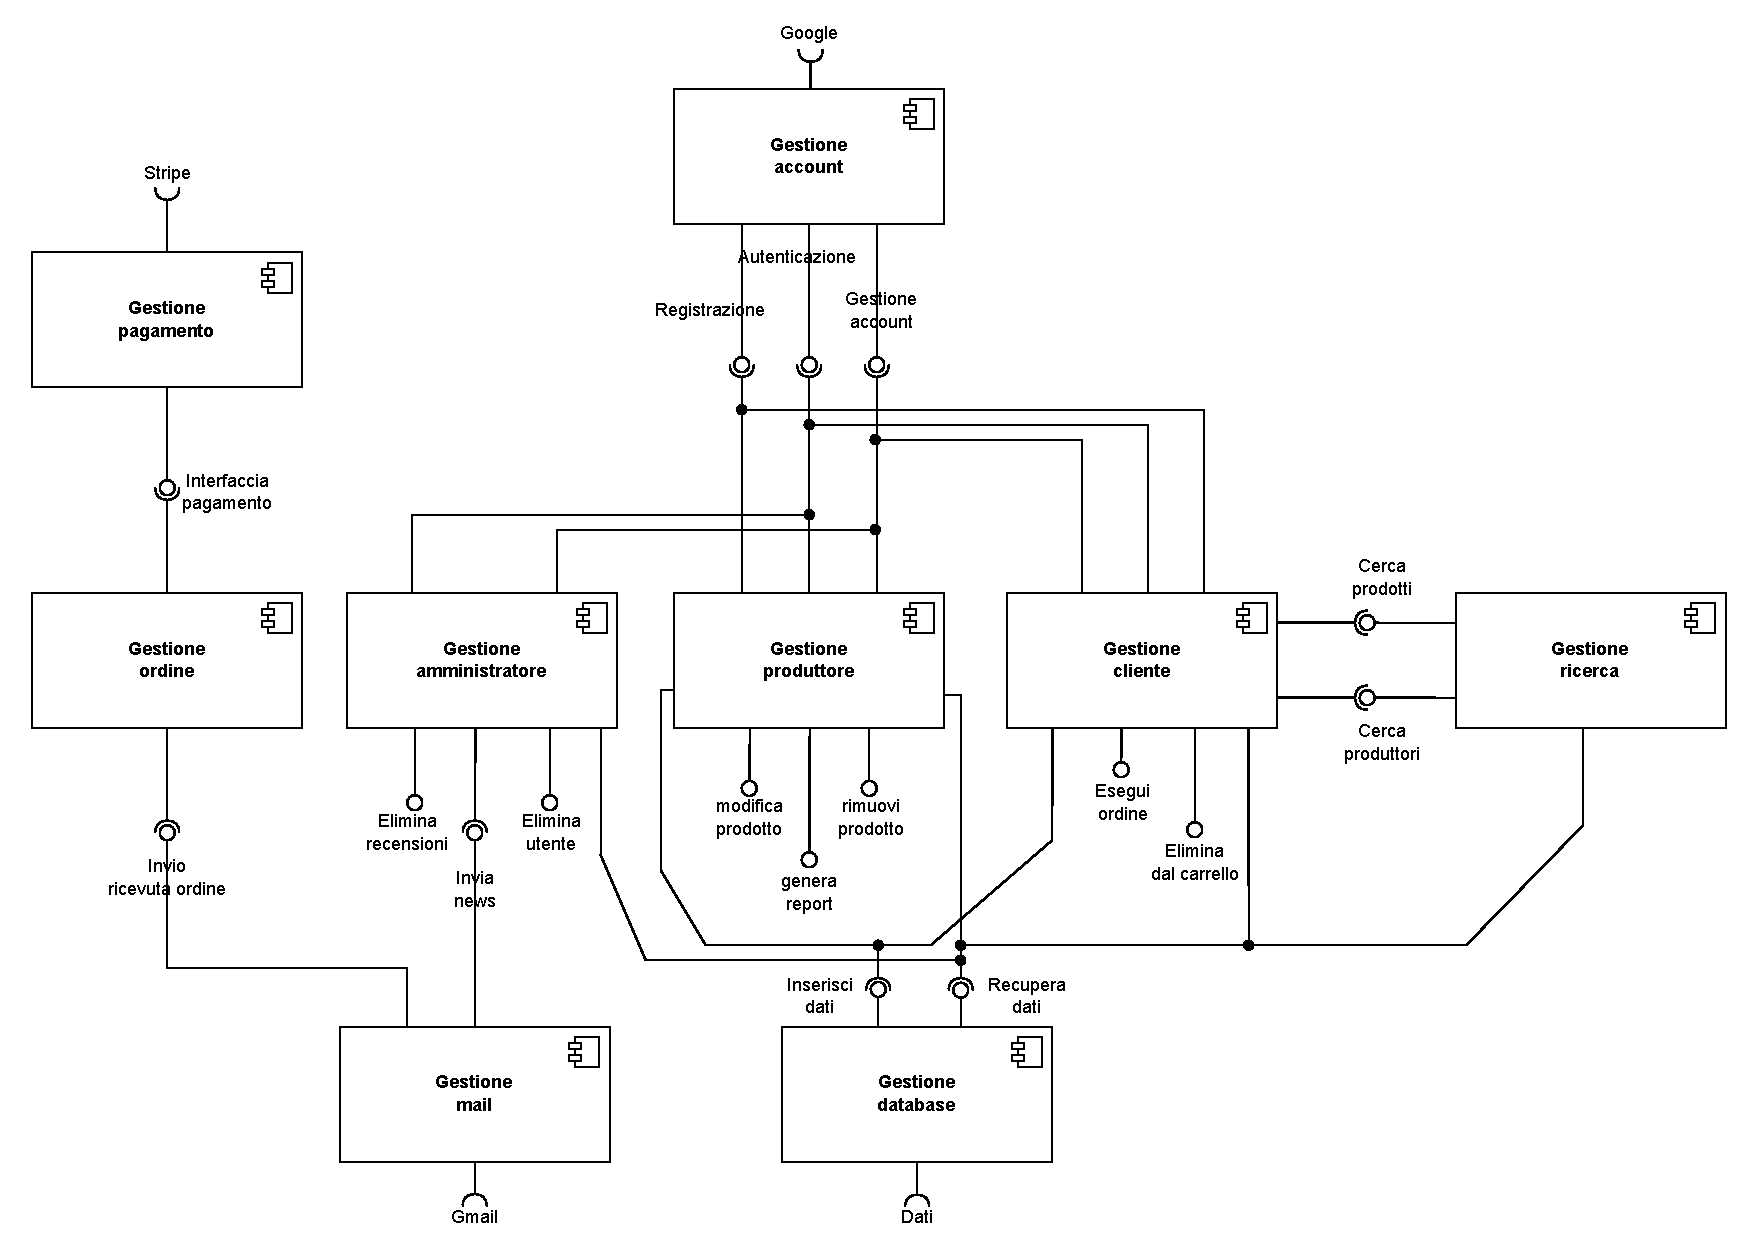
\includegraphics[trim= 0cm 0.2cm 0.4cm 0.3cm, clip, width=0.95\linewidth]{Deliverables/second-deliverable/img/Component-Diagram.drawio.pdf}
    \caption{Component diagram}
\end{figure}

\end{landscape}

\restoregeometry

\section{Diagramma dei componenti}

\subsection{Gestione account}
Questo componente gestisce tutta la complicazione della gestione degli account grazie all'utilizzo di Google Firebase.


\begin{table}[htbp!]
    \centering
    \begin{tabularx}{0.9\textwidth}{ >{\centering\arraybackslash}X | >{\centering\arraybackslash}X | m{8cm}}
        \hline
        \textbf{Tipologia} & \textbf{Nome}  & \textbf{Descrizione}\\
        \hline
        Fornita & Registrazione & Il componente fornisce un'interfaccia per registrare il proprio account nel sistema.\\
        \hline
        Fornita &  Autenticazione & Il componente fornisce un'interfaccia per autenticarsi nel sistema.\\
        \hline
        Fornita &  Gestione account & Il componente fornisce un'interfaccia per gestire il proprio account (es. Recupera password, elimina account)\\
        \hline
        Richiesta &  Google & Il componente utilizza un'interfaccia fornita da Google Firebase per fornire tutte le funzionalità \\
        \hline
    \end{tabularx}
    \caption{Gestione account}
    \label{tab:gestione-account}
\end{table}


\subsection{Gestione produttore}
Questo componente gestisce tutta l'interazione tra produttore ed applicazione.

\begin{table}[htbp!]
    \centering
    \begin{tabularx}{0.9\textwidth}{ >{\centering\arraybackslash}X | >{\centering\arraybackslash}X | m{8cm}}
        \hline
        \textbf{Tipologia} & \textbf{Nome}  & \textbf{Descrizione}\\
        \hline
        Fornita & Modifica prodotto & Il componente fornisce un'interfaccia modificare i dati del prodotto \\
        \hline
        Fornita & Genera report & Il componente fornisce un'interfaccia per generare un report per le statistiche.\\
        \hline
        Fornita &  Rimuovi prodotto & Il componente fornisce un'interfaccia per rimuovere un prodotto dallo store.\\
        \hline
        Richiesta &  Recupera dati & Il componente utilizza un'interfaccia fornita da Gestione database per recuperare tutti i dati necessari\\
        \hline
        Richiesta &  Inserisci dati & Il componente utilizza un'interfaccia fornita a Gestione database per inserire tutti i dati necessari\\
        \hline
        Richiesta &  Autenticazione & Il componente utilizza un'interfaccia fornita da Gestione account per autenticarsi nella piattaforma.\\
        \hline        
        Richiesta &  Gestione account & Il componente utilizza un'interfaccia fornita da Gestione account per gestire il proprio account.\\
        \hline
        Richiesta &  Registrazione & Il componente utilizza un'interfaccia fornita da Gestione account per registrarsi alla piattaforma.\\
        \hline
    \end{tabularx}
    \caption{Gestione produttore}
    \label{tab:gestione-produttore}
\end{table}

\newpage
\subsection{Gestione cliente}
Questo componente gestisce tutta l'interazione tra cliente ed applicazione.


\begin{table}[htbp!]
    \centering
    \begin{tabularx}{0.9\textwidth}{ >{\centering\arraybackslash}X | >{\centering\arraybackslash}X | m{8cm}}
        \hline
        \textbf{Tipologia} & \textbf{Nome}  & \textbf{Descrizione}\\
        \hline
        Fornita & Esegui ordine & Il componente fornisce un'interfaccia per eseguire un ordine.\\
        \hline
        Fornita & Elimina dal carrello & Il componente fornisce un'interfaccia per eliminare il prodotto dal carrello.\\
        \hline
        Richiesta &  Recupera dati & Il componente utilizza un'interfaccia fornita da Gestione database per recuperare tutti i dati necessari\\
        \hline
        Richiesta &  Inserisci dati & Il componente utilizza un'interfaccia fornita a Gestione database per inserire tutti i dati necessari\\
        \hline
        Richiesta &  Autenticazione & Il componente utilizza un'interfaccia fornita da Gestione account per autenticarsi nella piattaforma.\\
        \hline        
        Richiesta &  Gestione account & Il componente utilizza un'interfaccia fornita da Gestione account per gestire il proprio account.\\
        \hline
        Richiesta &  Registrazione & Il componente utilizza un'interfaccia fornita da Gestione account per registrarsi alla piattaforma.\\
        \hline
    \end{tabularx}
    \caption{Gestione cliente}
    \label{tab:gestione-cliente}
\end{table}

\subsection{Gestione ricerca}
Questo componente gestisce la ricerca all'interno della applicazione.


\begin{table}[htbp!]
    \centering
    \begin{tabularx}{0.9\textwidth}{ >{\centering\arraybackslash}X | >{\centering\arraybackslash}X | m{8cm}}
        \hline
        \textbf{Tipologia} & \textbf{Nome}  & \textbf{Descrizione}\\
        \hline
        Fornita & Cerca prodotti & Il componente fornisce un'interfaccia per cercare tutti i prodotti disponibili.\\
        \hline
        Fornita & Cerca produttori & Il componente fornisce un'interfaccia per cercare tutti i produttori disponibili.\\
        \hline
        Richiesta &  Recupera dati & Il componente utilizza un'interfaccia fornita da Gestione database per recuperare tutti i dati necessari\\
        \hline
    \end{tabularx}
    \caption{Gestione ricerca}
    \label{tab:gestione-ricerca}
\end{table}

\subsection{Gestione database}
Questo componente permette agli altri componenti di accedere in lettura e scrittura ai dati salvati nel database.


\begin{table}[htbp!]
    \centering
    \begin{tabularx}{0.9\textwidth}{ >{\centering\arraybackslash}X | >{\centering\arraybackslash}X | m{8cm}}
        \hline
        Fornita &  Recupera dati & Il componente fornisce un'interfaccia per recuperare tutti i dati salvati al suo interno.\\
        \hline
        Fornita &  Inserisci dati & Il componente fornisce un'interfaccia per inserire i dati che necessitano di persistenza.\\
        \hline
        Richiesta &  Dati & Il componente utilizza un'interfaccia fornita da MongoDB per inserire/recuperare i dati salvati.\\
        \hline
    \end{tabularx}
    \caption{Gestione database}
    \label{tab:gestione-database}
\end{table}


\subsection{Gestione mail}
Questo componente gestisce le interazioni con il sistema esterno Gmail.

\begin{table}[htbp!]
    \centering
    \begin{tabularx}{0.9\textwidth}{ >{\centering\arraybackslash}X | >{\centering\arraybackslash}X | m{8cm}}
        \hline
        \textbf{Tipologia} & \textbf{Nome}  & \textbf{Descrizione}\\
        \hline
        Fornita & Invio ricevuta ordine & Il componente fornisce un'interfaccia per inviare la ricevuta di ordine.\\
        \hline
        Fornita & Invia news & Il componente fornisce un'interfaccia per inviare le ultime news.\\
        \hline
        Richiesta &  Gmail & Il componente utilizza un'interfaccia fornita da Gmail per inviare le mail.\\
        \hline
    \end{tabularx}
    \caption{Gestione mail}
    \label{tab:gestione-mail}
\end{table}

\subsection{Gestione amministratore}
Questo componente gestisce la parte amministrativa del sistema.

\begin{table}[htbp!]
    \centering
    \begin{tabularx}{0.9\textwidth}{ >{\centering\arraybackslash}X | >{\centering\arraybackslash}X | m{8cm}}
        \hline
        \textbf{Tipologia} & \textbf{Nome}  & \textbf{Descrizione}\\
        \hline
        Fornita & Elimina recensioni & Il componente fornisce un'interfaccia per eliminare le recensioni che non rispettano le policy della piattaforma.\\
        \hline
        Fornita & Elimina utente & Il componente fornisce un'interfaccia per inviare le ultime news.\\
        \hline
        Richiesta & Invia news & Il componente fornisce un'interfaccia per inviare le ultime news.\\
        \hline
        Richiesta &  Autenticazione & Il componente utilizza un'interfaccia fornita da Gestione account per autenticarsi nella piattaforma.\\
        \hline        
        Richiesta &  Gestione account & Il componente utilizza un'interfaccia fornita da Gestione account per gestire il proprio account.\\
        \hline
    \end{tabularx}
    \caption{Gestione amministratore}
    \label{tab:gestione-amministratore}
\end{table}


\newpage
\subsection{Gestione ordine}
Questo componente gestisce gli ordini componendo anche un report da inviare tramite mail.

\begin{table}[htbp!]
    \centering
    \begin{tabularx}{0.9\textwidth}{ >{\centering\arraybackslash}X | >{\centering\arraybackslash}X | m{8cm}}
        \hline
        Richiesta &  Invio ricevuta ordine & Il componente utilizza un'interfaccia fornita da Gestione mail per inviare la ricevuta/fattura dell'ordine.\\
        \hline   
        Richiesta &  Interfaccia pagamento & Il componente utilizza un'interfaccia fornita da Gestione pagamento per ricevere la conferma ordine.\\
        \hline  
    \end{tabularx}
    \caption{Gestione ordine}
    \label{tab:gestione-ordine}
\end{table}


\subsection{Gestione pagamento}
Questo componente gestisce le interazioni con il sistema esterno Stripe.

\begin{table}[htbp!]
    \centering
    \begin{tabularx}{0.9\textwidth}{ >{\centering\arraybackslash}X | >{\centering\arraybackslash}X | m{8cm}}
        \hline
        \textbf{Tipologia} & \textbf{Nome}  & \textbf{Descrizione}\\
        \hline
        Fornita & Interfaccia pagamento & Il componente fornisce un'interfaccia per restituire tutti i dati necessari della transazione.\\
        \hline
        Richiesta &  Stripe & Il componente utilizza un'interfaccia fornita da Stripe per fornire il pagamento in-app.\\
        \hline    
    \end{tabularx}
    \caption{Gestione pagamento}
    \label{tab:gestione-pagamento}
\end{table}

